\documentclass[11pt]{article}

\usepackage{sectsty}
\usepackage{graphicx}
\usepackage{forest}
\usepackage{verbatim}
\usepackage[utf8]{inputenc}
\usepackage{tikz}
\usetikzlibrary{shapes.geometric, arrows}
\usepackage[hidelinks,pdfencoding=auto]{hyperref}
\usepackage{multirow}

% Margins
\topmargin=-0.45in
\evensidemargin=0in
\oddsidemargin=0in
\textwidth=6.5in
\textheight=9.0in
\headsep=0.25in

\title{Organisation of data in standardized HDF5 Brillouin spectra containers}
\author{Pierre Bouvet}
\date{\today}

\tikzstyle{startstop} = [rectangle, rounded corners, minimum width=3cm, minimum height=1cm,text centered, draw=black, fill=red!30]
\tikzstyle{io} = [trapezium, trapezium left angle=70, trapezium right angle=110, minimum width=3cm, minimum height=1cm, text centered, draw=black, fill=blue!30]
\tikzstyle{code} = [rectangle, minimum width=3cm, minimum height=1cm, text centered, draw=black]
\tikzstyle{process} = [rectangle, minimum width=3cm, minimum height=1cm, text centered, draw=black, fill=orange!30]
\tikzstyle{decision} = [diamond, minimum width=3cm, minimum height=1cm, text centered, draw=black, fill=green!30]
\tikzstyle{arrow} = [thick,->,>=stealth]

\begin{document}
\maketitle

\section{Introduction}

  The evolution of Brillouin Light Scattering (BLS) applications has lead to an increasing number of publications and research on this domain, resulting in a vast collection of data obtained with different techniques and setups by different laboratories. The evolution of this domain has reached the point where to allow it to grow outside of dedicated laboratories, a common approach to storing, treating and interpreting the data is needed. In an effort to facilitate this endeavour, we here propose a new normalized file structure based on the HDF5 file format, and introduce a dedicated Python Library: HDF5\_BLS to facilitate the use of the format and encourage its use as well as normalized treatment approaches.

  In this document, we will propose a normalized structure of the HDF5 files and present the concept behind the treatment of BLS spectra by the proposed Python library.

\section{Storing raw data in HDF5 wrapers}

  \subsection{Concept}

    The first need of the proposed format is to easily store data inside a HDF5 file. To do so, we propose to place the raw data in a dedicated object inside the HDF5 file, in the form of dataset:

    \begin{forest}
      for tree={font=\ttfamily, grow'=0, child anchor=west, parent anchor=south, anchor=west, calign=first,
        edge path={
          \noexpand\path [draw, \forestoption{edge}]
          (!u.south west) +(7.5pt,0) |- node[fill,inner sep=1.25pt] {} (.child anchor)\forestoption{edge label};
        },
        before typesetting nodes={
          if n=1
            {insert before={[,phantom]}}
            {}
        },
        fit=band,
        before computing xy={l=15pt},
      }
      [HDF5 file
        [Data (type: group)
        [Raw Data (type: Dataset)]
        ]
      ]
    \end{forest}

    From there the goal of the HDF5 file format is to store together with the data, the parameters used for the experiment. These parameters will be stored in the form of text attributes to the HDF5 file:

    \begin{forest}
      for tree={font=\ttfamily, grow'=0, child anchor=west, parent anchor=south, anchor=west, calign=first,
        edge path={
          \noexpand\path [draw, \forestoption{edge}]
          (!u.south west) +(7.5pt,0) |- node[fill,inner sep=1.25pt] {} (.child anchor)\forestoption{edge label};
        },
        before typesetting nodes={
          if n=1
            {insert before={[,phantom]}}
            {}
        },
        fit=band,
        before computing xy={l=15pt},
      }
      [HDF5 file
        [Attributes (type: HDF5 attributes stored as text)]
        [Data (type: group)
        [Raw Data (type: Dataset)]
        ]
      ]
    \end{forest}

    Because entering all the attributes of a spectrometer for each measure is time consuming, we propose to rely on a standardized spreadsheet that is imported to create the attributes. Aside from standardizing the nomenclature of the attributes, this will also allow researchers to create spreadsheets explicitely for their instrument, and reuse these documents each time the instrument is used for a new measure, with minimal changes. 

  \subsection{Use of the file format to wrap data}

    Using the proposed file structure allows us to add to the file, different data for different uses. For instance, a calibration curve of the spectrometer made with a sample of reference, a measure of its impulse response or any other data relevant to the experiment can be added to the file easily following this structure:

    \begin{forest}
      for tree={font=\ttfamily, grow'=0, child anchor=west, parent anchor=south, anchor=west, calign=first,
        edge path={
          \noexpand\path [draw, \forestoption{edge}]
          (!u.south west) +(7.5pt,0) |- node[fill,inner sep=1.25pt] {} (.child anchor)\forestoption{edge label};
        },
        before typesetting nodes={
          if n=1
            {insert before={[,phantom]}}
            {}
        },
        fit=band,
        before computing xy={l=15pt},
      }
      [HDF5 file
        [Attributes (type: HDF5 attributes stored as text)]
        [Data (type: group)
          [Raw spectrum (type: dataset)]
          [Calibration spectrum (type: dataset)]
          [Impulse response (type: dataset)]
          [Other data (type: dataset)]
        ]
      ]
    \end{forest}

    Creating different groups inside the same file can also be used to store data taken in different conditions. In that case, we propose to number the groups as follows:

    \begin{forest}
      for tree={font=\ttfamily, grow'=0, child anchor=west, parent anchor=south, anchor=west, calign=first,
        edge path={
          \noexpand\path [draw, \forestoption{edge}]
          (!u.south west) +(7.5pt,0) |- node[fill,inner sep=1.25pt] {} (.child anchor)\forestoption{edge label};
        },
        before typesetting nodes={
          if n=1
            {insert before={[,phantom]}}
            {}
        },
        fit=band,
        before computing xy={l=15pt},
      }
      [HDF5 file
        [Attributes (type: HDF5 attributes stored as text)]
        [Data (type: group)
          [Data\_0 (type: group)
            [Data\_0\_0 (type: group)
            [Data\_0\_0\_0 (type: group)]
            [Data\_0\_0\_1 (type: group)]
            [...]
            ]
            [Data\_0\_1 (type: group)]
            [...]
          ]
          [Data\_1 (type: group)]
          [...]
        ]
      ]
    \end{forest}

\section{Data types}

  To allow the storage of the largest type of data possible, we propose to store raw data as n-dimensional arrays of floating point numbers. This choice forces however to set a certain order on the dimensions, that we propose as follows:

  \begin{itemize}
    \item Nth dimension: spectral channels
    \item (N-1)th dimension: (if reported) z dependence
    \item (N-2)th dimension: (if reported) y dependence
    \item (N-3)th dimension: (if reported) x dependence
    \item (N-4)th dimension: (if reported) time dependence
    \item (N-5)th dimension: (if reported) radial angular dependence
    \item (N-6)th dimension: (if reported) azimutal angular dependence
    \item (N-7)th dimension: (if reported) temperature dependence
    \item (N-8)th dimension: (if reported) concentration dependence
    \item (N-9)th dimension and further: user-specific dimensions
  \end{itemize}

  We propose that in case of redundancy (for example a dependance on both time and position), the user chooses the relevant dimension.

\section{List of attributes}

One key condition for this format to be useful for meta-studies, is to allow users to access the same parameters of the measures in different files. To do so, we propose a normalization of the name of the attributes. This list will evolve and can be found on the dedicated GitHub page of the project in "spreadsheets/attributes.xlsx".

These attributes are divided in three sections:
\begin{itemize}
  \item Measure: all the parameters that are measure-dependent and that are not strictly linked to the tool used to measure the BLS spectra
  \item Spectrometer: all the parameters that are instrument-dependent. This includes all the choices made at the moment of developping the spectrometer. This separation is particularly interesting for manufacturers of standard tools as they can directly refer the model of their device here and adapt their treatments to this single parameter. 
  \item File properties: all the file-related parameters that are linked to the numerical storage of the data and are not dependent neither on the measure nor the instrument.
\end{itemize}

This list is prone to evolve and we encourage everyone interested in this project to share with us the parameters they feel are needed for their particular application in order to add it to the standard. 

\section{HDF5\_Brillouin\_creator modules structure}

    The module presented here aims at allowing the user to import, convert, organize and treat the data. As such the module is divided in four sub-modules:
    \begin{itemize}
      \item load\_data: the sub-module dedicated to extract data and attributes from a file.
      \item wraper: the sub-module dedicated to creating the object where both the data and attributes will be stored, where the treatment steps will be recorded and that can export to a HDF5 file.
      \item pre\_treat: the sub-module dedicated to obtain a BLS spectrum from the raw data, a step dependent on the type of technique and the spectrometer being used to acquire the spectrum.
      \item treat: the sub-module dedicated to treating a Brillouin spectrum.
    \end{itemize}

    The library is meant for unifying the storage and treatment of spectra which can be schematized by the following pipeline:\\


    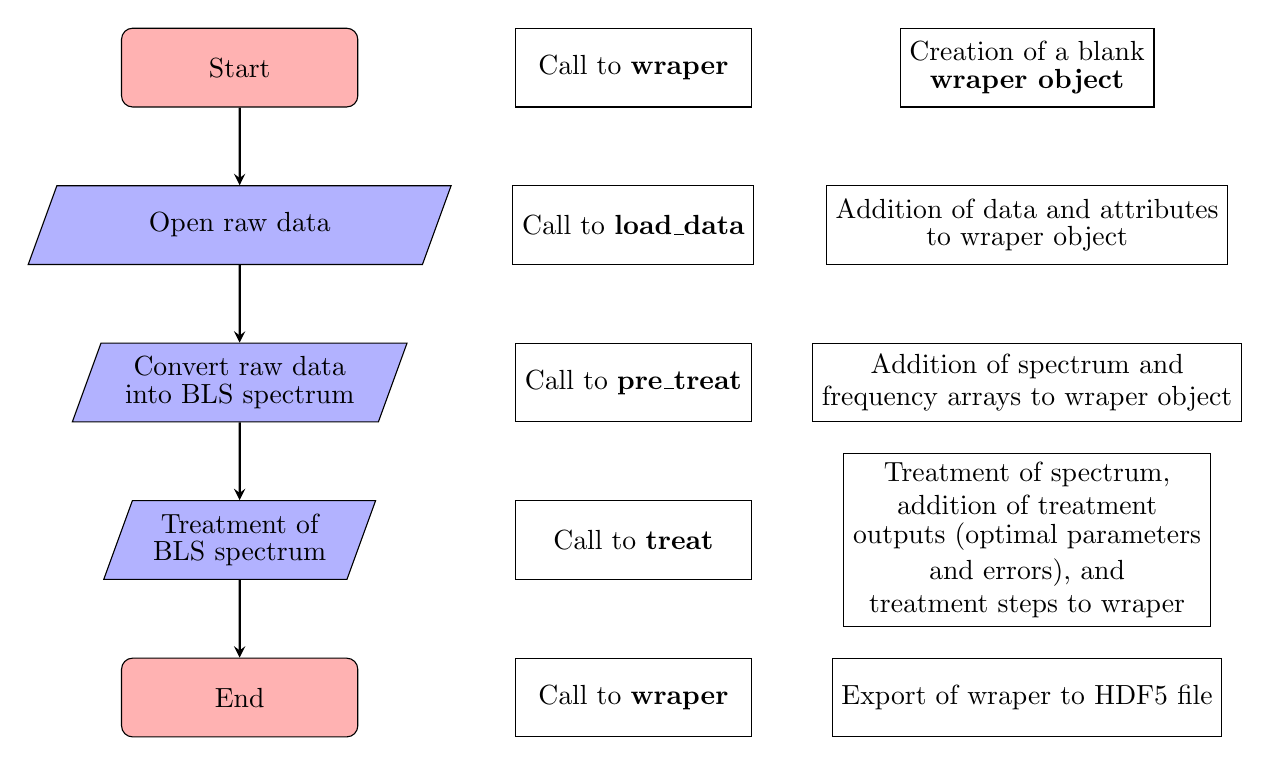
\begin{tikzpicture}[node distance=2cm]
      \node (start) [startstop] {Start};
      \node (inc0) [code, right of=start, xshift=3cm] {Call to \bf{wraper}};
      \node (inw0) [code, right of=inc0, xshift=3cm] {\shortstack{Creation of a blank \\ \bf{wraper} object}};
      \node (in1) [io, below of=start] {Open raw data};
      \node (inc1) [code, right of=in1, xshift=3cm] {Call to \bf{load\_data}};
      \node (inw1) [code, right of=inc1, xshift=3cm] {\shortstack{Addition of data and attributes \\ to wraper object}};
      \draw [arrow] (start) -- (in1);
      \node (in2) [io, below of=in1] {\shortstack{Convert raw data \\ into BLS spectrum}};
      \node (inc2) [code, right of=in2, xshift=3cm] {Call to \bf{pre\_treat}};
      \node (inw2) [code, right of=inc2, xshift=3cm] {\shortstack{Addition of spectrum and \\ frequency arrays to wraper object}};
      \draw [arrow] (in1) -- (in2);
      \node (in3) [io, below of=in2] {\shortstack{Treatment of \\ BLS spectrum}};
      \node (inc3) [code, right of=in3, xshift=3cm] {Call to \bf{treat}};
      \node (inw3) [code, right of=inc3, xshift=3cm] {\shortstack{Treatment of spectrum, \\ addition of treatment \\ outputs (optimal parameters \\ and errors), and \\ treatment steps to wraper}};
      \draw [arrow] (in2) -- (in3);
      \node (stop) [startstop, below of=in3] {End};
      \draw [arrow] (in3) -- (stop);
      \node (inc4) [code, right of=stop, xshift=3cm] {Call to \bf{wraper}};
      \node (inw4) [code, right of=inc4, xshift=3cm] {\shortstack{Export of wraper to HDF5 file}};
    \end{tikzpicture}

\section{Independent use of the module}
  
  The module can be used independently of the wraper module, by simply calling the desired functions of the three sub-modules "load\_data", "pre\_treat" and "treat".

\end{document}
